\chapter{Signals processing and classification of data force}
\label{ch:forceData}

\section{Introduction and chapter's structure}
In the previous chapter, we analysed and extracted features of force data and inertial sensors data of the patients from the same experiment . Thus, once we compared both systems and determined the relationship between them, we proceed to conclude whether we can classify force data from patients and control subjects.

Along this chapter, we are going to explain Hardware used in this experiment, the procedure to gathering the data, the process carried out to calculate the relevant signals, different techniques to feature extraction as well as the results obtained after the classification of this information.

\section{PLS}
Partial least squares regression (PLS regression) is a statistical method that bears some relation to principal components regression; instead of finding hyperplanes of minimum variance between the response and independent variables, it finds a linear regression model by projecting the predicted variables and the observable variables to a new space \cite{pls_pca} 
%\cite{pls_wiki}.

This algorithm is based on linear transition from a large number of original descriptors to a new variable space based on small number of orthogonal factors (latent variables), i.e factors are mutually independent (orthogonal) linear combinations of original descriptors\cite{pls_pca} .
%\cite{pls}.

We used in the last chapter PCA algorithm to extract features of the gait data. This new method is very similar but there are clear differences. Both PCA and PLS are used as a dimension reduction methodology. However, PCA is applied without the consideration of the correlation between the dependent variable and the independent variables, while PLS is applied based on the correlation. Therefore, we call PCA as an unsupervised dimension reduction methodology, and call PLS as a supervised dimension reduction methodology, i.e it has a phase of training and another of evaluation or testing\cite{pls_pca}.

Once establish the most important differences between them, we are going to explain the fundamentals of this algorithm. 
Assume X is a \textit{n×p} matrix and Y is a \textit{n×q} matrix. The PLS technique works by successively extracting factors from both X and Y such that covariance between the extracted factors is maximized. In our particular case, we will assume that we have a single response variable i.e., Y is \textit{n×1} and X is \textit{n×p}, as before.

\begin{center}
	$ Y= UQ’+F $

$ X=TP’+E $
\end{center}

where Q\textit{(qxr)} and P \textit{(pxr)} are the matrices of coefficients (orthogonal loading matrices) , F \textit{(nxq)} and E \textit{(nxp)} are the error term and, U \textit{(nxr)} and T \textit{(nxr)} matrices that are, respectively, projections of X and projections of Y.

Decomposition is finalized so as to maximize covariance between T and U. All algorithms to solve this follow an iterative process to extract the T(X-scores) and U(Y-scores)\cite{pls_pca}. 

The factors or scores for X and Y are extracted successively and the number of factors extracted \textit{(r)} depends on the rank of X and Y. In our case, Y is a vector and all possible X factors will be extracted.
Each extracted X-score are linear combinations of X. Thus, the score T of X is of the form: 

\begin{center}
	$ T= XW $
\end{center}

Where  W is a matriz obtained as follow:

\begin{center}
	$ W= conv(X,Y); $
$ W = W/||W|| $
\end{center}

With r (latents variables) columns.

\section{Signals processing and feature extraction}
The database used in this experiment  is different in contrast with the above case. This contains measure of gait from 27 patients (mean age: 66.3 years; 63 \% men) and 18 healthy controls (mean age: 66.3 years; 63\% men). The database includes the vertical ground reaction force records of subjects as they walked at their usual. They wear underneath each foot 8 sensors\cite{Instr6} that measure force as a function time. The output of each of these 16 sensors has been digitized and recorded at 100 samples per second.

Once data have been gathered while subjects were walking during two minutes approximately, we read this information from the text file. This file contains the force of each sensors as well as the sum of force of the right and left feet.

With these values, we can obtain the center of pressure Antero-Posterior and Medio-Lateral  as indicate the equation \ref*{COP}. To do this, we have to define the position of the sensors. When a person is comfortably standing with both legs parallel to each other, sensor locations inside the insole can be described (according to \cite{Instr6}) as lying approximately at the following (X,Y) coordinates, assuming that the origin (0,0) is just between the legs and the person is facing towards the positive side of the Y axis:
\begin{figure}[H]
	\centering
	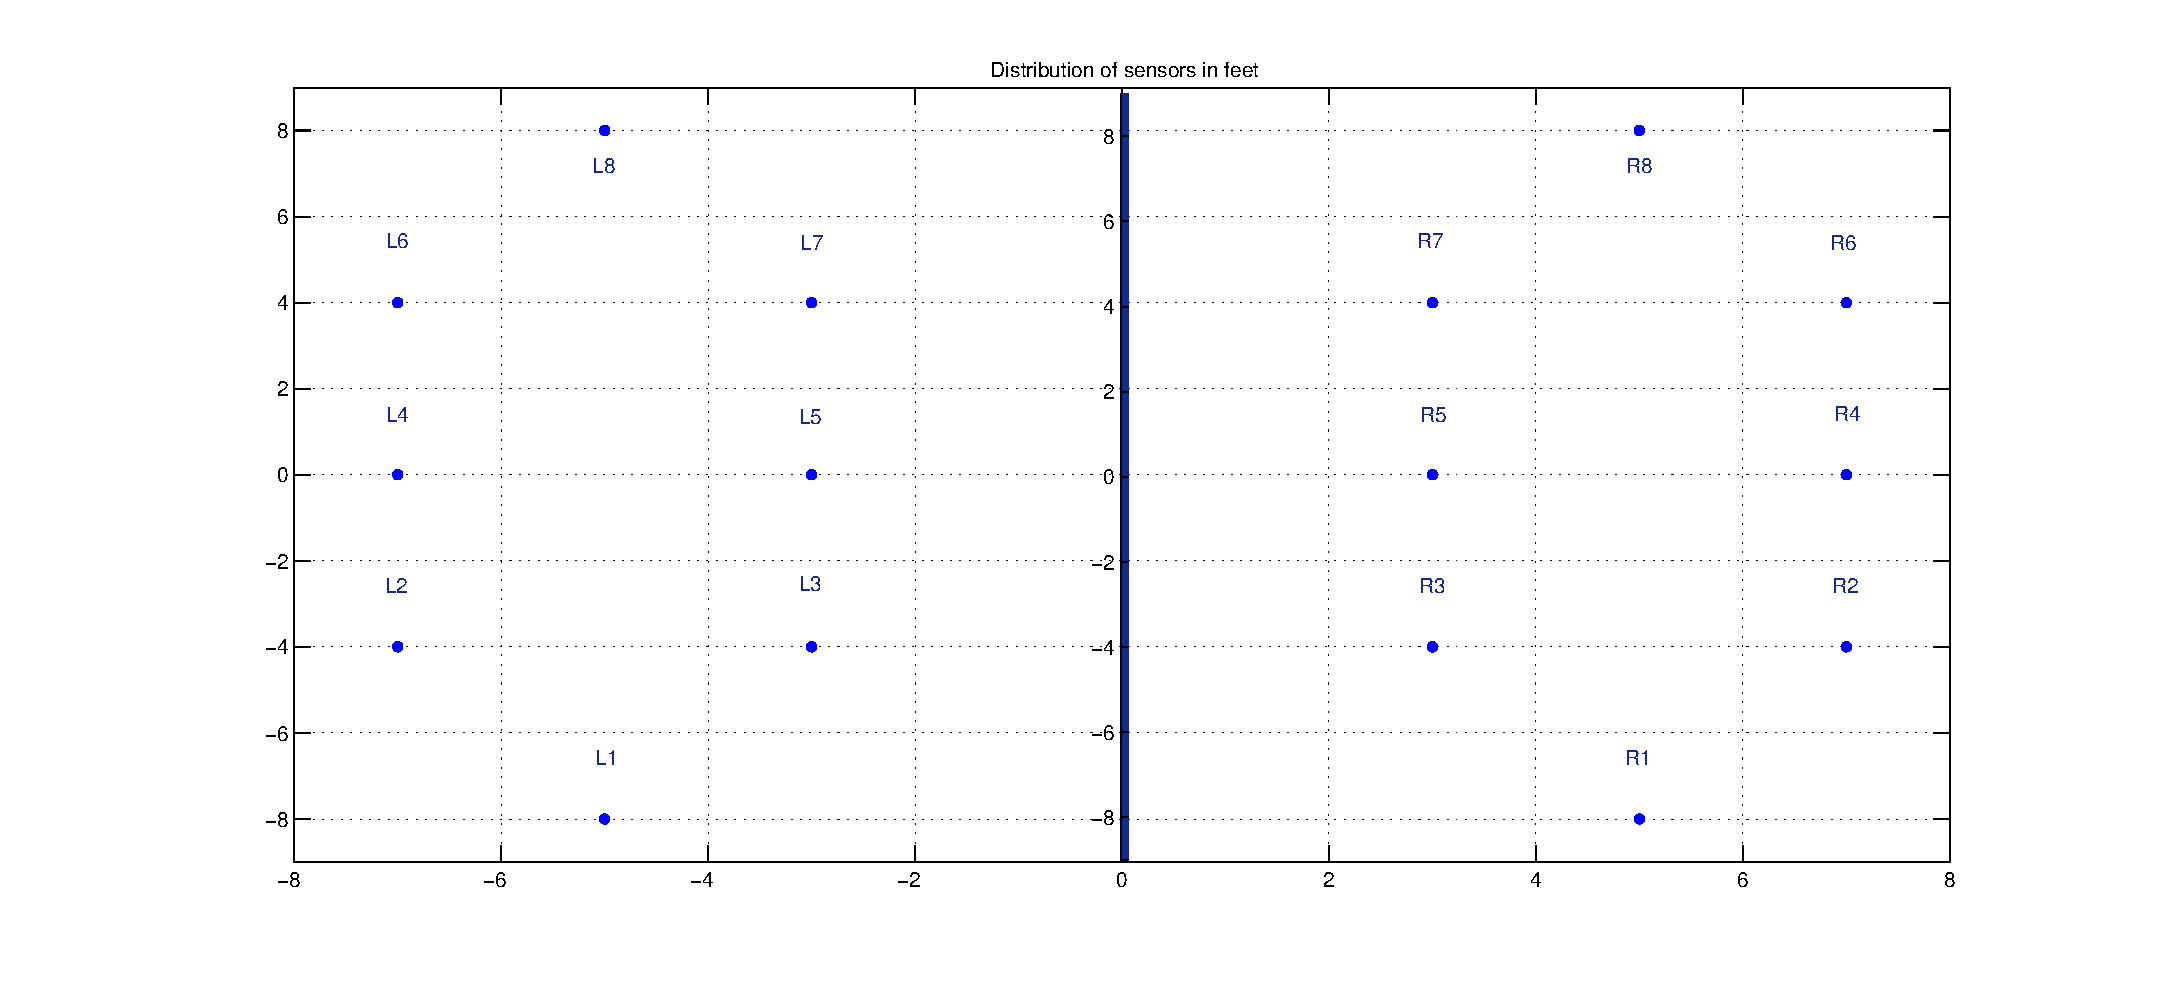
\epsfig{file=figures/forceData/DistributionSensors, width=18cm}
	\caption{Distribution of the sensors underneath both feet.}
	\label{fig:DistributionSensors}
\end{figure}

The X and Y numbers are in an arbitrary coordinate system reflecting the relative (arbitrarily scaled) positions of the sensors within each insole. During walking, the sensors inside each insole remain at the same relative position, but the two feet are no longer parallel to each other. Thus, this coordinate system enables a calculation of a proxy for the location of the center of pressure (COP) under each foot.

Hereafter, we separate the differents steps because the subjects carry out several steps during the experiment. We detect this when the COP signal has a strong fall in one of the feet. One we have delimited the intervals of the signals, we figure out the average of them using cross correlation to synchronise the cycles properly. We can see the result in the following figure:
\begin{figure}[H]
	\centering
	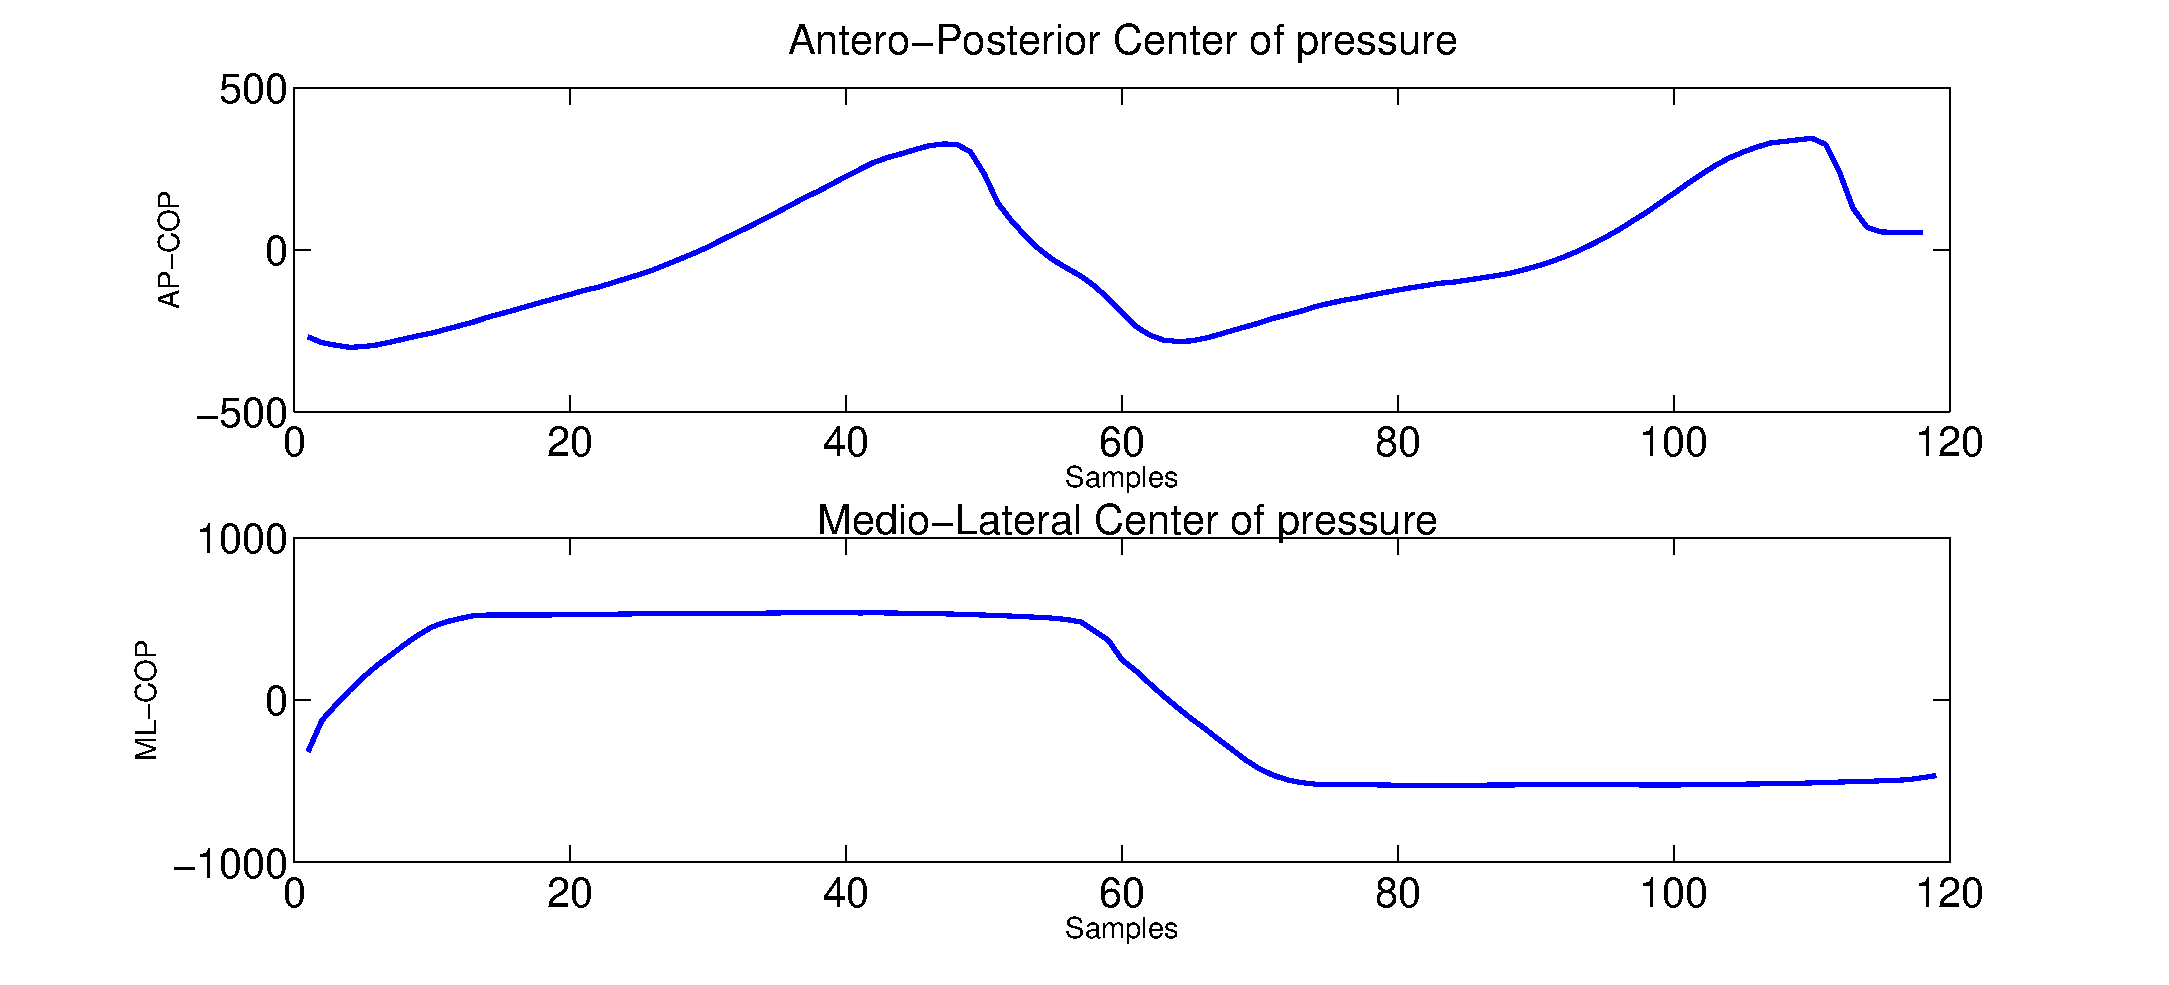
\epsfig{file=figures/forceData/COP, width=18cm}
	\caption{Center of pressure in AP and ML direction.}
	\label{fig:COP}
\end{figure}

Thus, after this, we only have two signals ML and AP COP that represent one step of the patient. It is not absolutely necessary but it allows us to obtain a average of each repeat, being this more appropriate to characterise the subjects.

We use these signals to apply PCA as in the previous experiment. We match ML-COP and AP COP in the same column corresponding to the same subject and rearrange both patients and healthy controls in the same data matrix to apply this algorithm.

As we explained before, PCA is an unsupervised method\ref{fig:PCA}, so we will use PLS algorithm to extract the relevant information and carry out a better classification of the data. We calculated X-score of the all data for different numbers of components (latent variables). The results after the classification can be seen in the next section.

\begin{figure}[H]
	\centering
	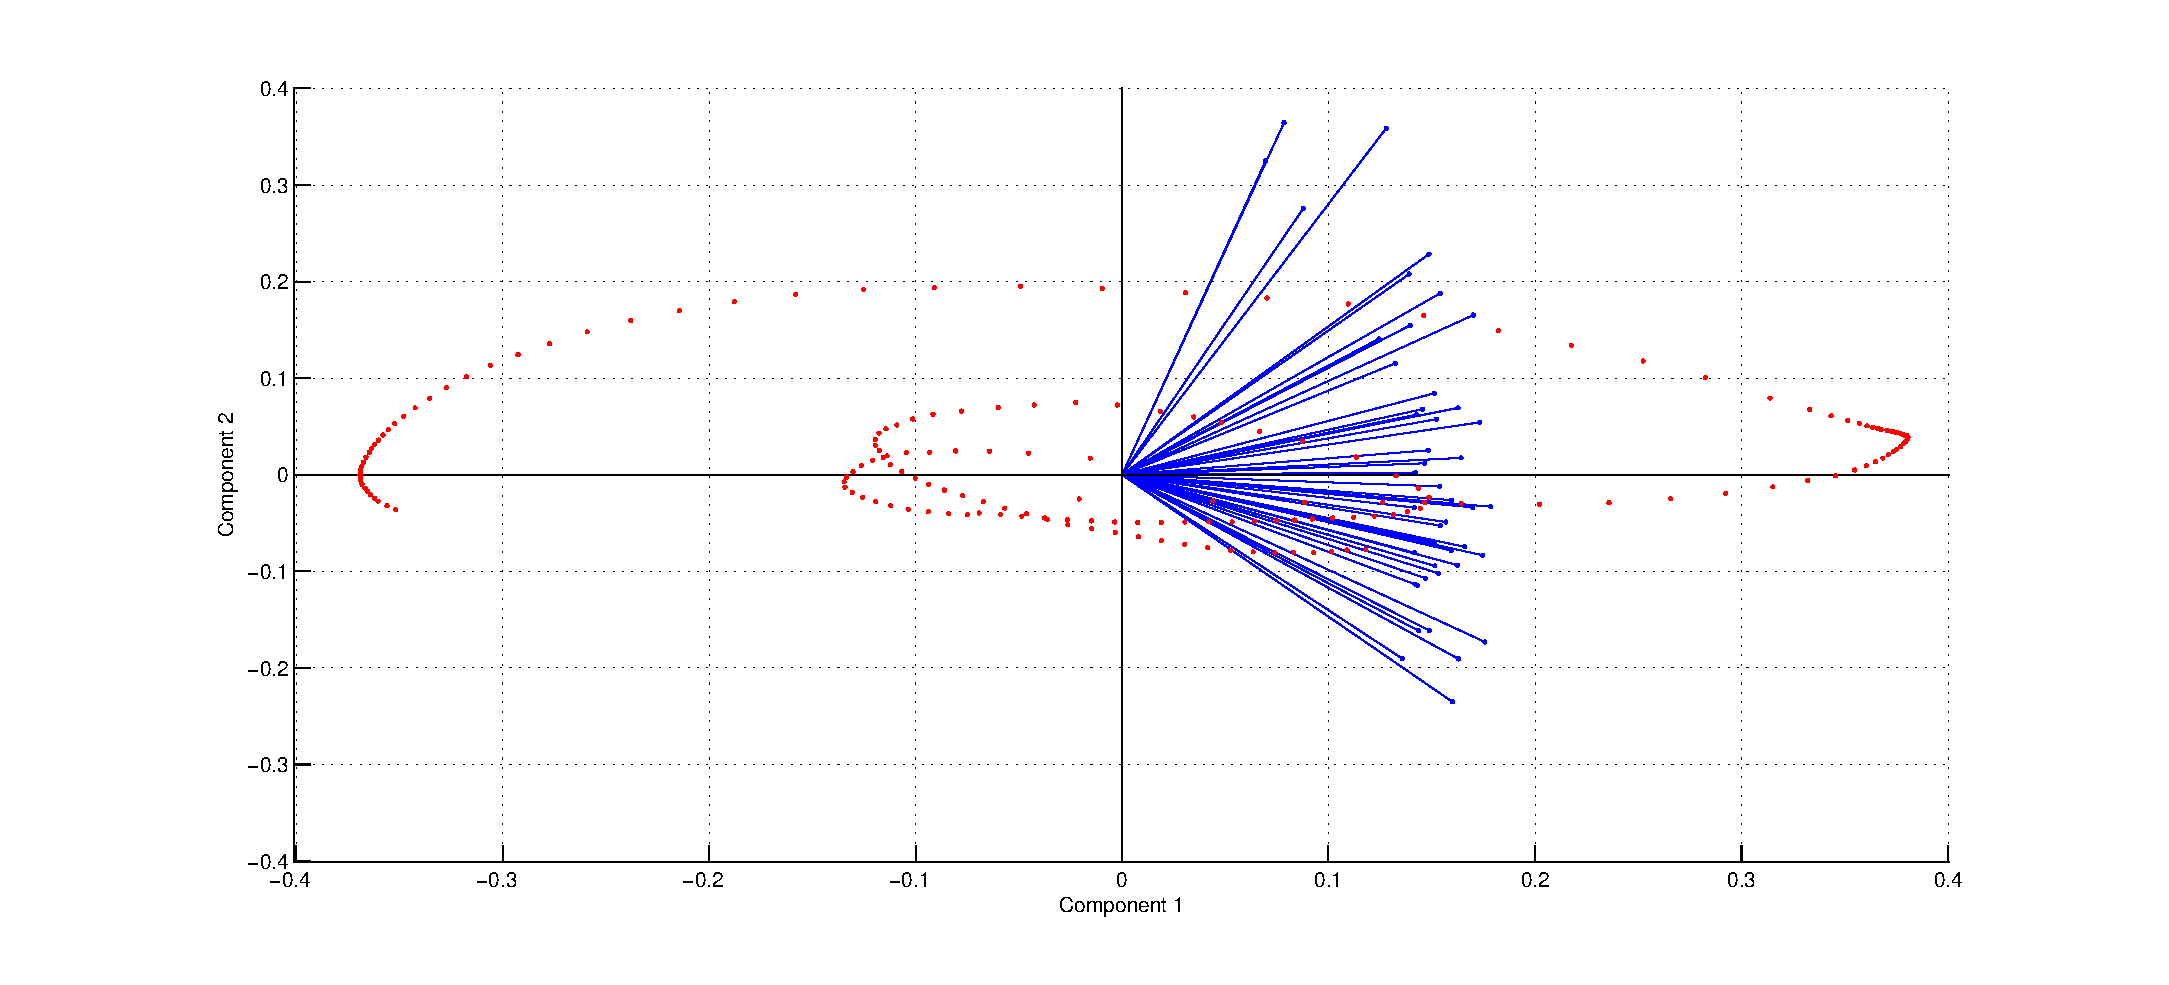
\epsfig{file=figures/forceData/PCA, width=18cm}
	\caption{PCA applied for all subjects}
	\label{fig:PCA}
\end{figure}

\section{Classification and Results discurssion}

Once we used PCA and PLS algorithm for feature extration, we have the relevant information to classify. This classification is carried out using support vector machine classifier (SVM).

This method separates a given set of binary labelled training data with a hyperplane that is maximally distant from the two classes (known as the maximal margin hyperplane). The objective is to build a function \textit{(f)} using training data (x,y) \cite{Gorriz}.
 
Thus, f will correctly classify new examples (x, y). When no linear separation of the training data is possible, SVMs can work effectively in combination with kernel techniques using the kernel trick, so that the hyperplane defining the SVMs corresponds to a nonlinear decisión boundary in the input space that is mapped to a linearised higherdimensional space . In this way the decision function f can be expressed in terms of the support vectors only\cite{Gorriz}:

\begin{center}
	$f(x) = sign{\sum_{i=1}^{N} \alpha_{i}y_{i}K(s_{i},x)}$
\end{center}

Where $K$ is a kernel function, $\alpha$ is a weight constant derived from the SVM process and the $s_{i}$ are the support vectors. 

In our particular case, the testing was carried off with ‘Leave-One-Out’ technique, i.e in every iteration where the training was realised, one of the subjects was used for testing. . In addition, several Kernel were used in this checking, specifically a linear kernel \textit{(‘linear’)}, Quadratic kernel \textit{(‘Quadratic’)}, polynomial kernel of order 3 \textit{(‘polynomial’)} and a Gaussian Radial Basis Function kernel\textit{('rbf')} with a scaling factor of 1.

Firstly, we use SVM over PLS data with differents components. As we said in the PLS chapter, the rank of latent variables depends on the input data. There is a number of components which the results is more accurate and the results after the classification is better. Thus, we represent the accuracy, sensibility and specificity as function of the number of components and in turn for differents kernel functions. This allows us determine the best number of components and  kernel that we can use.

If we observe the figure \ref{fig:stadistics_PLS}, we can fix that ,for our data, the \textit{‘linear’} and \textit{‘rbf’} functions with seven and two components respectively are the best options to do the classification because the reparation in the space with them allows to classify these data with more precision.  In addition, the accuracy is 86.67\%, so we can conclude that the classification is precise and optimal and also one possible method to medical diagnostic.

\begin{figure}[H]
	\centering
	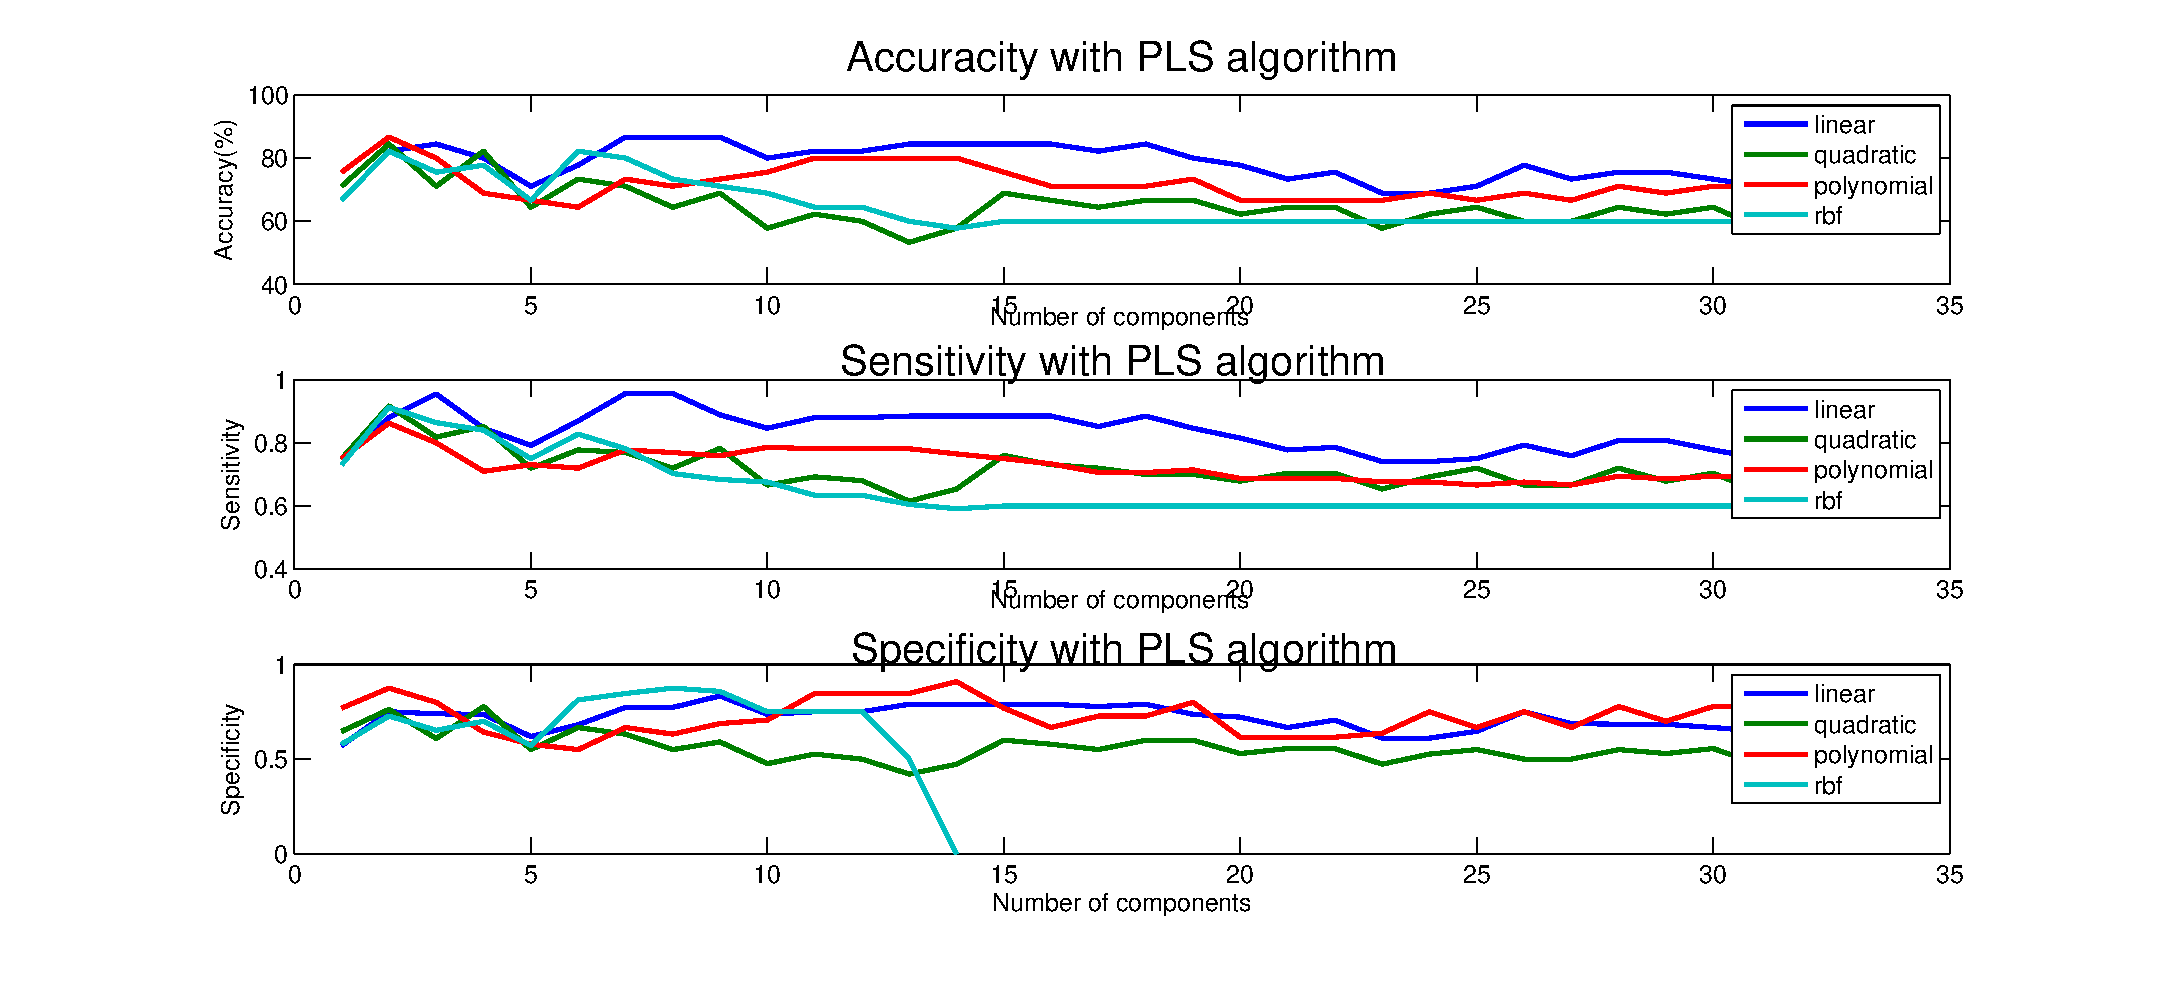
\epsfig{file=figures/forceData/stadistics_PLS, width=18cm}
	\caption{Stadistics with PLS data after used SVM to classify.}
	\label{fig:stadistics_PLS}
\end{figure}

This can be seen in these 3D representations \ref{} \ref{} where it is shown the points used to the classification as well as the kernel function for the two best cases, i.e \textit{‘linear’} and \textit{‘rbf’} functions.

\begin{figure}[H]
	\centering
	\epsfig{file=figures/forceData/Classification3D_PLS_linear, width=18cm}
	\caption{Classification of PLS data with the 'linear' kernel.}
	\label{fig:Classification3D_PLS_linear}
\end{figure}

\begin{figure}[H]
	\centering
	\epsfig{file=figures/forceData/Classification3D_PLS_rbf, width=18cm}
	\caption{Classification of PLS data with the 'rbf' kernel.}
	\label{fig:Classification3D_PLS_rbf}
\end{figure}

Thereupon, we will do the classification from PCA data. To do this, firstly we select the components that explain the most of variability\ref{fig:variance_PCA}.

\begin{figure}[H]
	\centering
	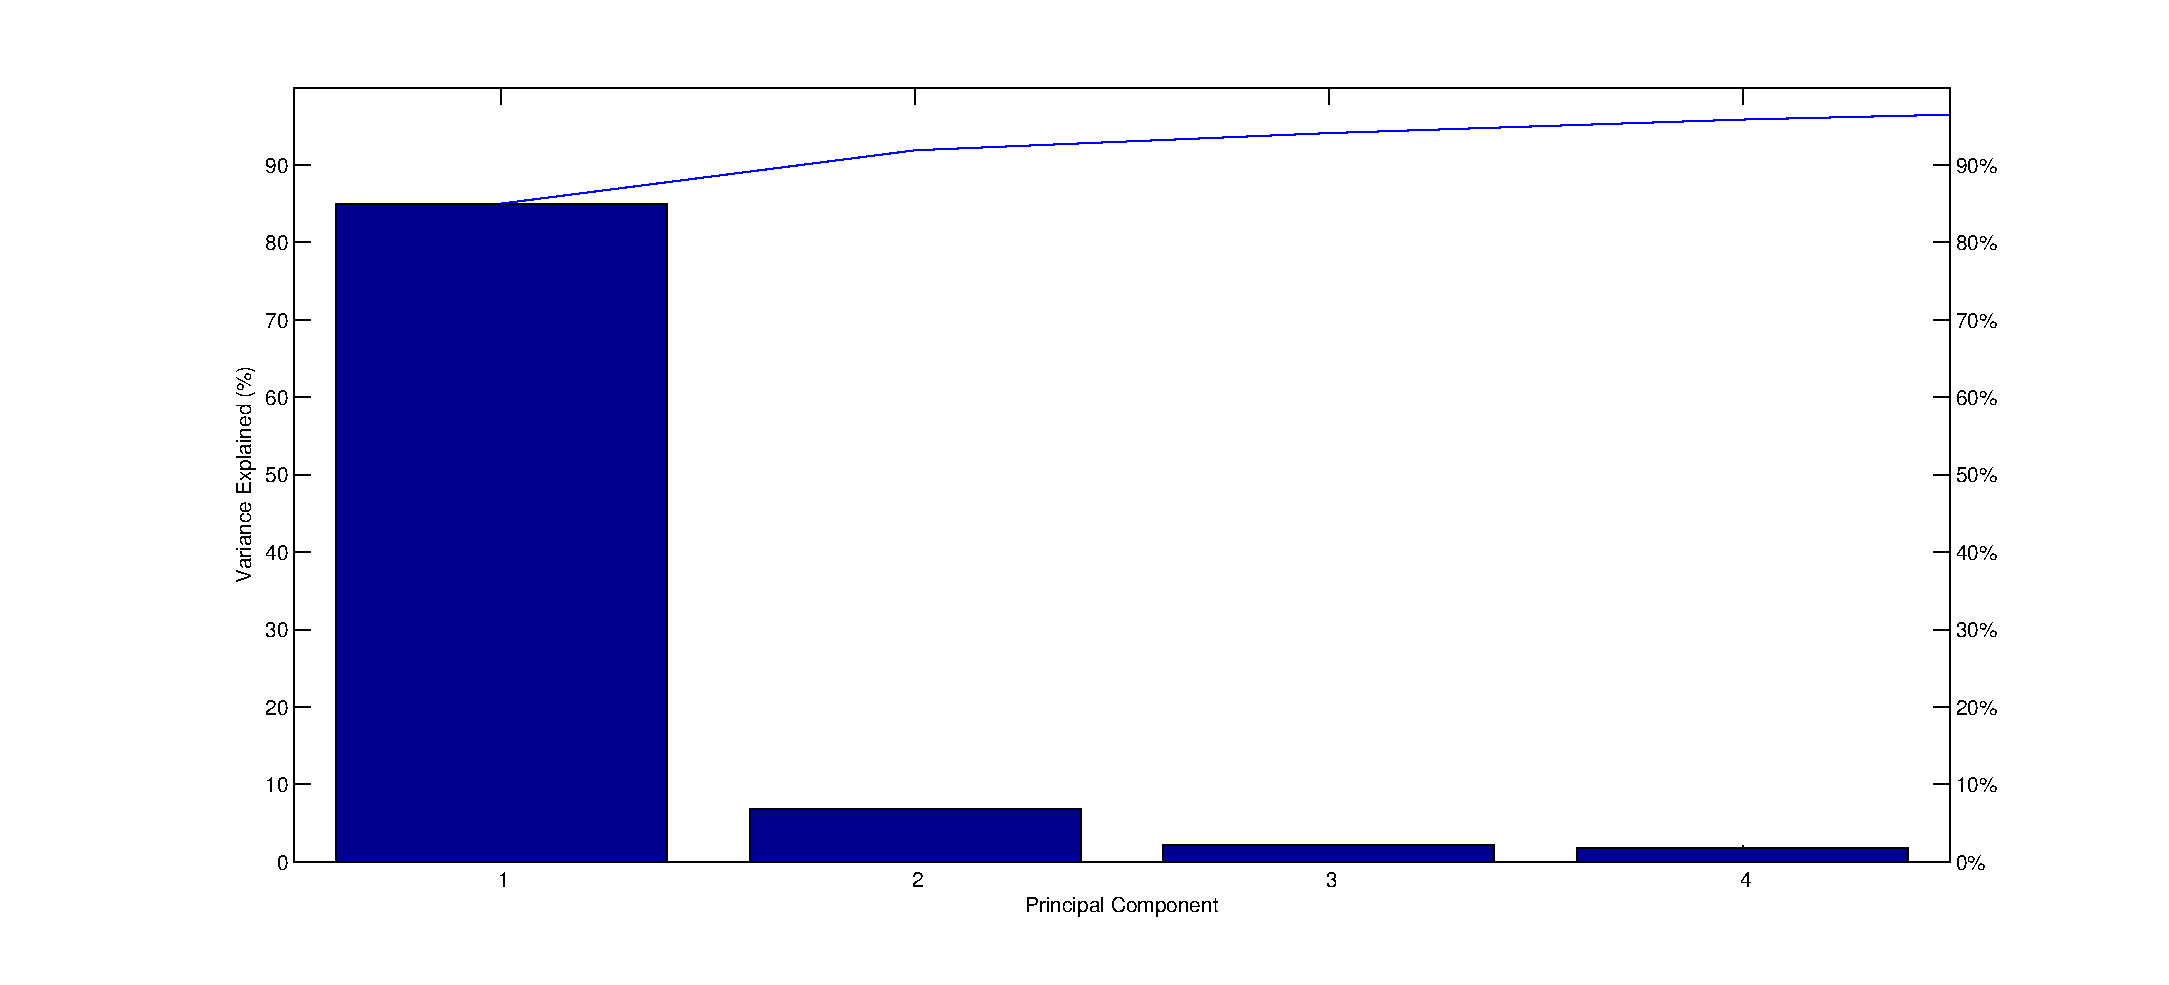
\epsfig{file=figures/forceData/variance_PCA, width=18cm}
	\caption{Variance explained for PCA algorithm.}
	\label{fig:variance_PCA}
\end{figure} 

The above scree plot only shows the first four (instead of the total forty-five) components that explain 95\% of the total variance. The only clear break in the amount of variance accounted for by each component is the first component, explaing about 85\% of the variance, so any more components might be needed, so it is  a reasonable way to reduce the dimensions.

Then, we will apply SVM over data for the rank of components between one and four, achieving 91\% of accuracy for ‘linear’ kernel function\ref{fig:stadistics_PCA}. Thus, we can obtain even more precision with this method. It makes sense because the four first components explain the majority of variance.

\begin{figure}[H]
	\centering
	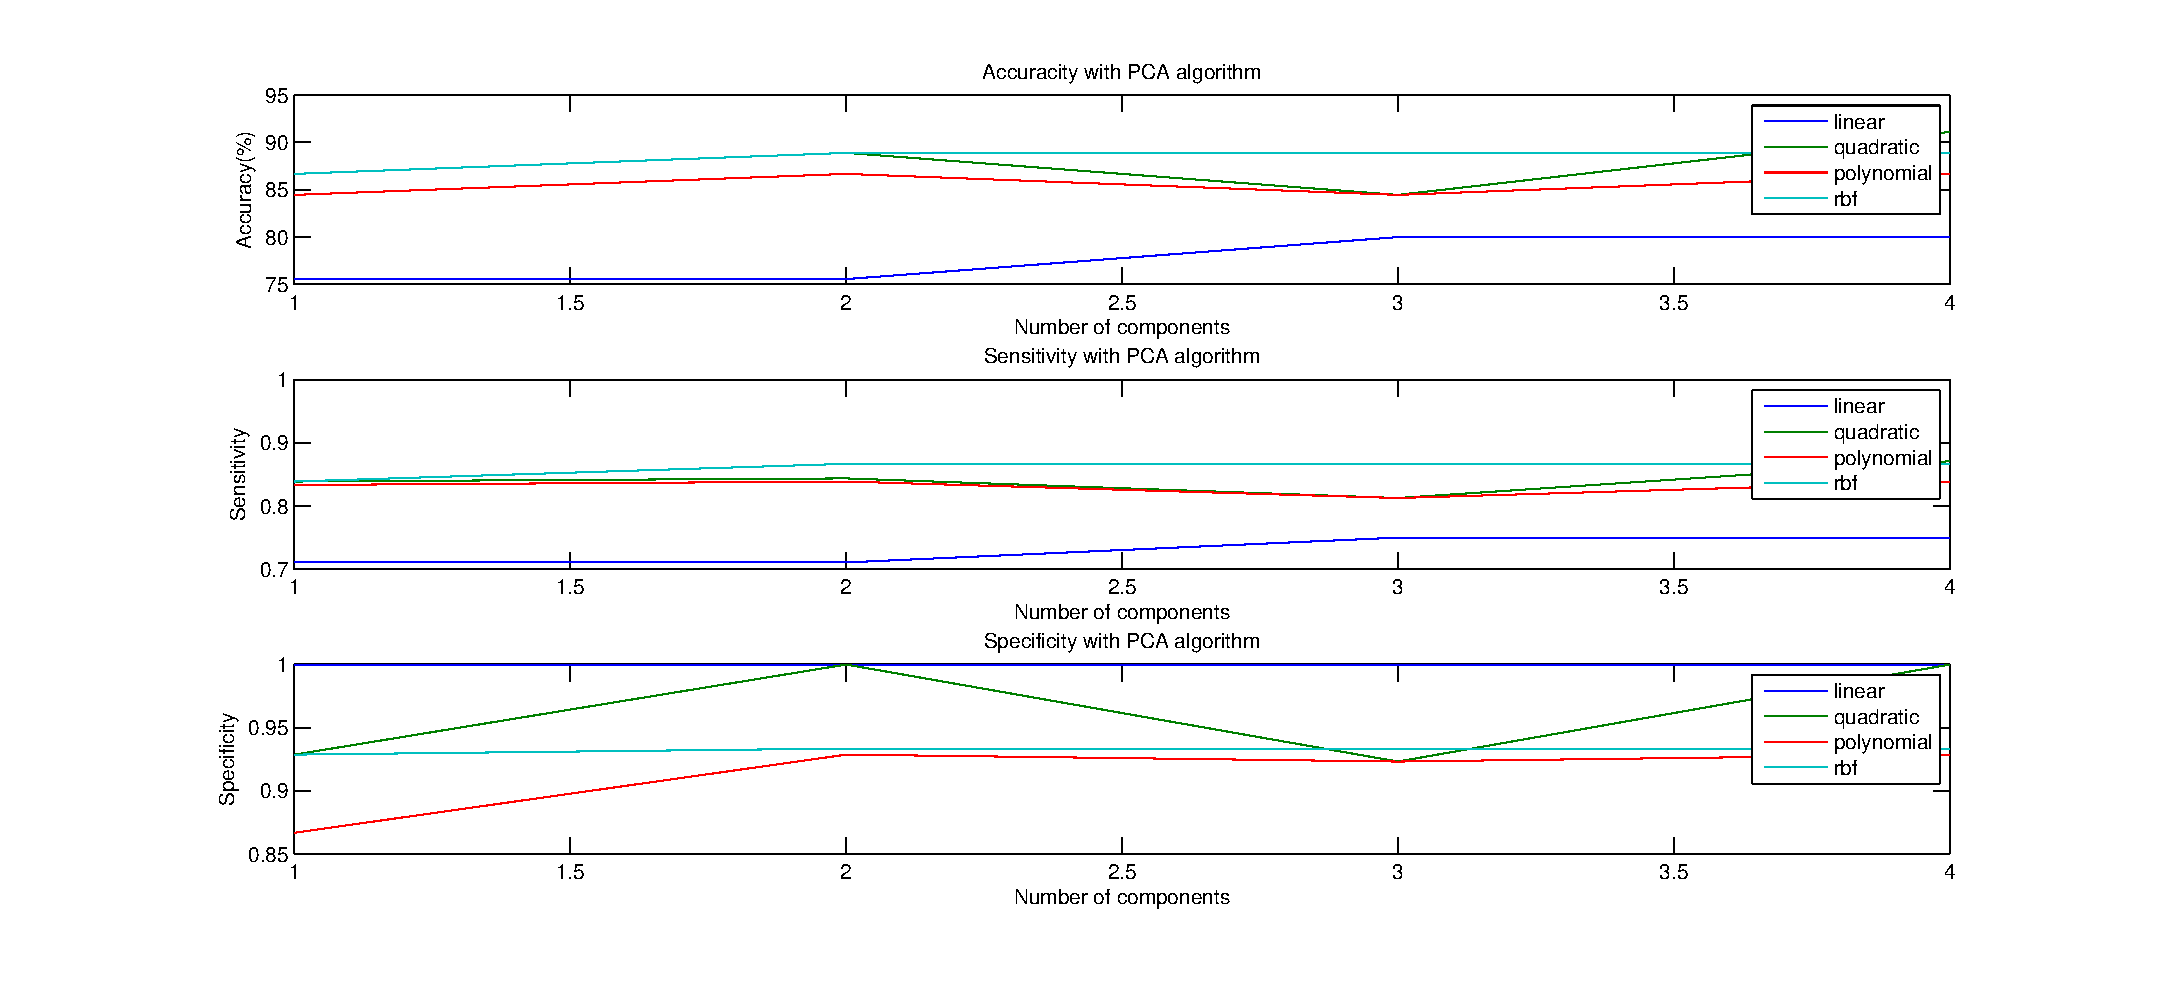
\epsfig{file=figures/forceData/stadistics_PCA, width=18cm}
	\caption{Stadistics with PCA data after used SVM to classify.}
	\label{fig:stadistics_PCA}
\end{figure}

Also, we can see the result of the classification in the following figure:

\begin{figure}[H]
	\centering
	\epsfig{file=figures/forceData/Classification3D_PCA, width=18cm}
	\caption{Classification of PCA data with the 'linear' kernel.}
	\label{fig:Classification3D_PCA}
\end{figure}

Finally, we will draw the ROC curve (Receiver Operating Characteristic). It  is a graphical plot that illustrates the performance of a binary classifier system as its discrimination threshold is varied. The curve is created by plotting the true positive rate against the false positive rate\cite{ROC1}.

The true-positive rate (TPR) is also known as sensitivity. The TPR defines how many correct positive results occur among all positive samples available during the test. In our particular case, it measures how many patients are recognised as such.

The false-positive rate (FPR) is also known as the fall-out and can be calculated as 1 - specificity. It defines how many incorrect positive results occur among all negative samples available during the test, in other words, how many patients are identified as heathy people.
The best possible prediction method would yield a point in the upper left corner or coordinate (0,1) of the ROC space, representing 100\% sensitivity (no false negatives) and 100\% specificity (no false positives). The (0,1) point is also called a \textit{perfect classification}. A completely random guess would give a point along a diagonal line (the so-called line of \textit{no-discrimination}) from the left bottom to the top right corners (regardless of the positive and negative base rates). The diagonal divides the ROC space. Points above the diagonal represent good classification results (better than random), points below the line poor results (worse than random)\cite{ROC1}.

The ROC is used to generate a summary statistic. One of the most common and useful measures is \textit{‘Area Under Curve’} (AUC) that is equal to the probability that a classifier will rank a randomly chosen positive instance higher than a randomly chosen negative one (assuming 'positive' ranks higher than 'negative'). A rough guide for classifying the accuracy of a diagnostic test is the traditional academic point system\cite{ROC2}:

0.90 - 1 = excellent (A)

0.80 - 0.90 = good (B)	

0.70 - 0.80 = fair (C)

0.60 - 0.70 = poor (D)

0.50 - 0.60 = fail (F)

Thus, if we represent the ROC curve using the force data after applying PLS and PCA with a SVM classifier (using a ‘linear’ kernel), we can see that the ROC curve with PLS is over PCA-ROC curve\ref{fig:ROC}.
\begin{figure}[H]
	\centering
	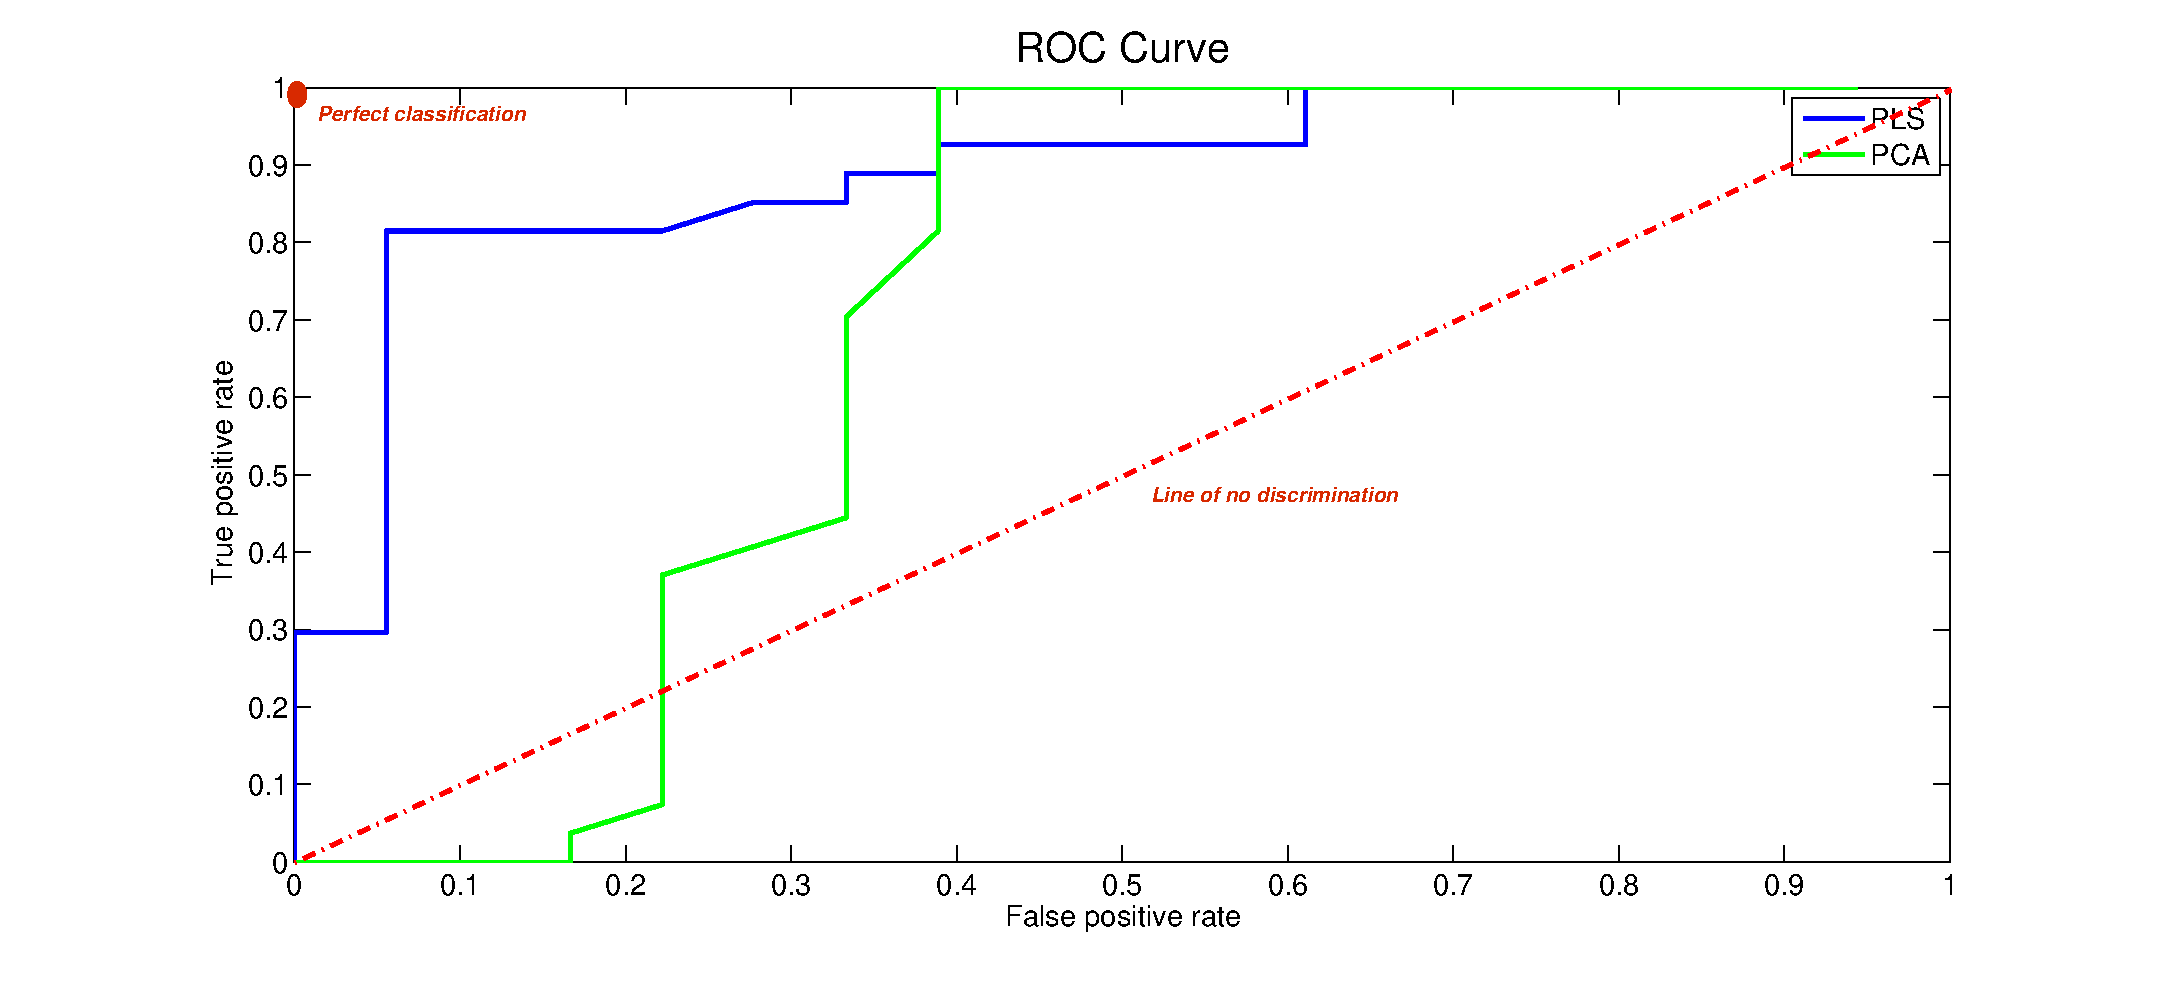
\epsfig{file=figures/forceData/ROC, width=18cm}
	\caption{ROC Curve for PLS and PCA with SVM classifier.}
	\label{fig:ROC}
\end{figure}

Also, if we calculate the AUC, we obtain that with PLS this value is 0.8344, so the classification is good. However, using PCA data, the AUC has a value of 0.6461, that is tos ay, it is a poor classification.

In a nutshell, from a accuracy viewpoint, PCA works better than PLS. Nevertheless, PLS is better in terms of sensibility, obtaining a great difference with regard to PCA as we can appreciate if we compare the AUC values. Thus, we can conclude that, in general terms, PLS could give us a better results because the difference in accuracy is less than the difference in ROC analysis. 
